%%
% Template for Assignment Reports
% 
%

\documentclass{article}

\usepackage{fancyhdr} % Required for custom headers
\usepackage{lastpage} % Required to determine the last page for the footer
\usepackage{extramarks} % Required for headers and footers
\usepackage{graphicx,color}
\usepackage{anysize}
\usepackage{amsmath}
\usepackage{natbib}
\usepackage{caption}
\usepackage{hyperref}
\usepackage{listings}
\usepackage{float}
\usepackage{lipsum}  
\usepackage{xcolor}
\usepackage{subcaption}
\usepackage{listings}
\usepackage{color}

\definecolor{dkgreen}{rgb}{0,0.6,0}
\definecolor{gray}{rgb}{0.5,0.5,0.5}
\definecolor{mauve}{rgb}{0.58,0,0.82}

\lstset{frame=tb,
  language=Java,
  aboveskip=3mm,
  belowskip=3mm,
  showstringspaces=false,
  columns=flexible,
  basicstyle={\small\ttfamily},
  numbers=none,
  numberstyle=\tiny\color{gray},
  keywordstyle=\color{blue},
  commentstyle=\color{dkgreen},
  stringstyle=\color{mauve},
  breaklines=true,
  breakatwhitespace=true,
  tabsize=3
}

% Margins
%\topmargin=-0.45in
%\evensidemargin=0in
%\oddsidemargin=0in
\textwidth=6.5in
%\textheight=9.0in
%\headsep=0.25in 

\linespread{1.0} % Line spacing

\definecolor{codegreen}{rgb}{0,0.6,0}
\definecolor{codegray}{rgb}{0.5,0.5,0.5}
\definecolor{codepurple}{rgb}{0.58,0,0.82}
\definecolor{backcolour}{rgb}{0.95,0.95,0.92}

\lstdefinestyle{mystyle}{
    backgroundcolor=\color{backcolour},   
    commentstyle=\color{codegreen},
    keywordstyle=\color{magenta},
    numberstyle=\tiny\color{codegray},
    stringstyle=\color{codepurple},
    basicstyle=\ttfamily\footnotesize,
    breakatwhitespace=false,         
    breaklines=true,                 
    captionpos=b,                    
    keepspaces=true,                 
    numbers=left,                    
    numbersep=5pt,                  
    showspaces=false,                
    showstringspaces=false,
    showtabs=false,                  
    tabsize=2
}

\lstset{style=mystyle}

%%------------------------------------------------
%% Image and Listing code
%%------------------------------------------------
%%sw \includecode{caption for table of listings}{caption for reader}{filename}
\newcommand{\includecode}[3]{\lstinputlisting[float,floatplacement=H, caption={[#1]#2}, captionpos=b, frame=single]{#3}}


%%sw \includescalefigure{label}{short caption}{long caption}{scale}{filename}
\newcommand{\includescalefigure}[5]{
\begin{figure}[htb]
\centering
\includegraphics[width=#4\linewidth]{#5}
\captionsetup{width=.8\linewidth} 
\caption[#2]{#3}
\label{#1}
\end{figure}
}

%%sw \includefigure{label}{short caption}{long caption}{filename}
\newcommand{\includefigure}[4]{
\begin{figure}[htb]
\centering
\includegraphics{#4}
\captionsetup{width=.8\linewidth} 
\caption[#2]{#3}
\label{#1}
\end{figure}
}




%%------------------------------------------------
%% Parameters
%%------------------------------------------------
% Set up the header and footer
\pagestyle{fancy}
\lhead{\authorName} % Top left header
\chead{\moduleCode\ - \assignmentTitle} % Top center header
\rhead{\firstxmark} % Top right header
\lfoot{\lastxmark} % Bottom left footer
\cfoot{} % Bottom center footer
\rfoot{Page\ \thepage\ of\ \pageref{LastPage}} % Bottom right footer
\renewcommand\headrulewidth{0.4pt} % Size of the header rule
\renewcommand\footrulewidth{0.4pt} % Size of the footer rule
\setlength\parindent{0pt} % Removes all indentation from paragraphs

\newcommand{\assignmentTitle}{Lab 4} % Assignment title
\newcommand{\moduleCode}{CSU44061} 
\newcommand{\moduleName}{Machine Learning} 
\newcommand{\authorName}{Adriana\ Hrabowych} % Your name
\newcommand{\authorID}{19304296} % Your student ID
\newcommand{\reportDate}{\printDate}

%%------------------------------------------------
%%	Title Page
%%------------------------------------------------
\title{
\vspace{-1in}
\begin{figure}[!ht]
\flushleft

\includegraphics[width=0.4\linewidth]{reduced-trinity.png}
\end{figure}
\vspace{-0.5cm}
\hrulefill \\
\vspace{0.5cm}
\textmd{\textbf{\moduleCode\ \moduleName}}\\
\textmd{\textbf{\assignmentTitle}}\\
\vspace{0.5cm}
\hrulefill \\
}

\author{\textbf{\authorName,\ \authorID}}

\date{\today}



%%------------------------------------------------
%% Document
%%------------------------------------------------
\begin{document}
\lstset{language=Java, captionpos=b, frame=single, keywordstyle=\color{black}\bfseries, stringstyle=\ttfamily}
\captionsetup{width=.8\linewidth} 

\maketitle


%%------------------------------------------------

\section{Part i }

\subsection{(i)(a)}
Convolving is the process of applying a kernel or filter to an input matrix to produce an output matrix. It is a process used in Convolutional Networks usually for image processing. 

In this part I coded a function to achieve convolution, it assumes a step of 1 and doesn't add any padding to the input matrix. The convolve function I coded takes an input matrix of size n x n and an input kernel of size k x k. The size of the output matrix is determined by:
\begin{center}
Output Height = Input Height - Kernel Height + 1

Output Width = Input Width - Kernel Width + 1
\end{center}
Using a helper function, the kernel is transformed into a 1D array with the 1st row being followed by the second row, followed by the third, and so on. 

\begin{lstlisting}
for i in range(rows):
     for j in range(cols):
         arrnn = squareTo1D(nn, len(kk), len(kk[0]), i, j)
         num = 0
         for k in range(len(arrnn)):
             num = num + (arrnn[k] * arrkk[k])
         output[i][j] = num
return output
\end{lstlisting}
Then, for each index in the output array a square of size k is taken from the input array with the index being the top left corner. This square is converted to a 1D array using a helper function. The sum of each index in this array being multiplied with the same index in the kernel array is then mapped to the output array. 

\subsection{(i)(b)}

\begin{center}

\includegraphics[width=.2\linewidth]{../triangle.png}
\end{center}
\captionof{figure}{An image of a blue triangle on a white background. It is 200 pixels squared in size.}

\begin{center}
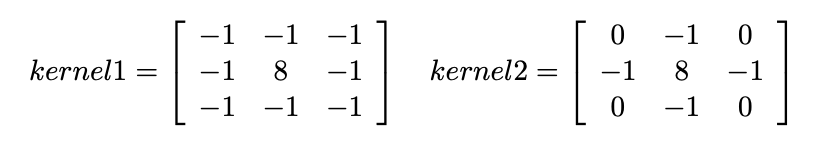
\includegraphics[width=.6\linewidth]{k.png}
\end{center}
\captionof{figure}{An image containing two kernel matrices, labelled kernel1 and kernel2.}

First we translate our image into a black and white pixel array. A visualization of the pixel array can be seen in figure 3(a). Using our convolve function we apply the two kernels in figure 2 onto the image in figure 1, the outcomes of which can be seen in figures 3 (b) and (c).

\begin{figure}[H]
\centering
\begin{subfigure}{.3\linewidth}
  \centering
  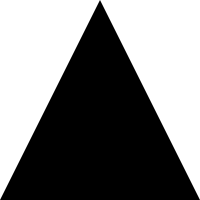
\includegraphics[width=\linewidth, height=4cm]{ib1.png}
  \caption{Blue triangle image converted to pixel array.}
  \label{fig:sub1}
\end{subfigure}%
\begin{subfigure}{.3\textwidth}
  \centering
  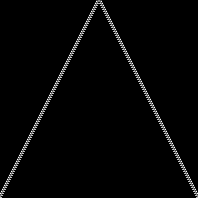
\includegraphics[width=\linewidth, height=4cm]{ib2.png}
  \caption{Subfigure (a) filtered using kernel1.}
  \label{fig:sub2}
\end{subfigure}
\label{fig:test}
\begin{subfigure}{.3\linewidth}
  \centering
  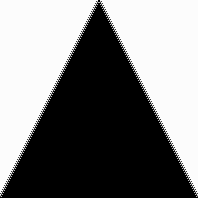
\includegraphics[width=\linewidth, height=4cm]{ib3.png}
  \caption{Subfigure (a) filtered using kernel2.}
  \label{fig:sub3}
\end{subfigure}%
\caption{A figure with three subfigures, each containing a filtered image of the triangle in figure 1 visualizing part ib of the lab. }
\label{fig:test}
\end{figure}

Kernel1 is used to detect the edges between areas with drastically different levels of greyness, like the boundaries of a shape. As seen in figure 3(b), only the edge of the original triangle is outputted in white. Kernel2 is used to detect ridges/different areas of an image, like the shape of an object. In figure 3(c) the background is outputted in white while the original is left black to represent different areas.

\subsection{(ii)(a)}
The Convnet used in the code takes an input of size (32x32x3). This input is then put through a convolution layer with an output filter size of 16, this increases the number of channels in the output to 16 creating an output shape of (32x32x16). Then theres another convolution layer, again with a filter size of 16 but this time with a stride size of (2,2). This increase in stride from the default (1,1) causes the output width and height of the output to decrease creating an output shape of (16x16x16). Next is a convolution layer with a stride of (1,1) and a filter size of 32, increasing the amount of channels again to an output shape of (16x16x32). The final convolution layer has a filter size of 32 and a stride (2,2), this increase stride once again halves the output width and height leaving an output shape of (8x8x32). Each of these convolution layers used a kernel of size (3,3).

Next is a dropout layer with a parameter drop rate of 0.5. A dropout layer is only used in training, and prevents overfitting. Nothing in this layer changes the output shape. Then there is a flatten layer, this layer flattens the data into a 1D vector. The output shape is therefore just a vector of size 8 * 8 * 32 = 2048.

Finally the vector is put through a dense layer which maps and connects the 2048 inputs to 10 outputs, as specified. 

\subsection{(ii)(b)(i)}
Keras says the model has 37,146 total parameters, the layer with the most parameters is the dense layer which has 20,490 parameters total. The dense layer is a network layer, it connects every single pixel from its input to a number output classes (defined as ten outputs in the code). This is a lot of links to make and as such it requires a lot of parameters.

The f1 score of the model on the training data was 0.64, and on the testing data it was 0.50. For comparison, a randomly predicting dummy had an f1 score of 0.10 for both sets. The model performed better on the training data than on testing data, and the dummy in both.

\subsection{(ii)(b)(ii)}
\begin{center}
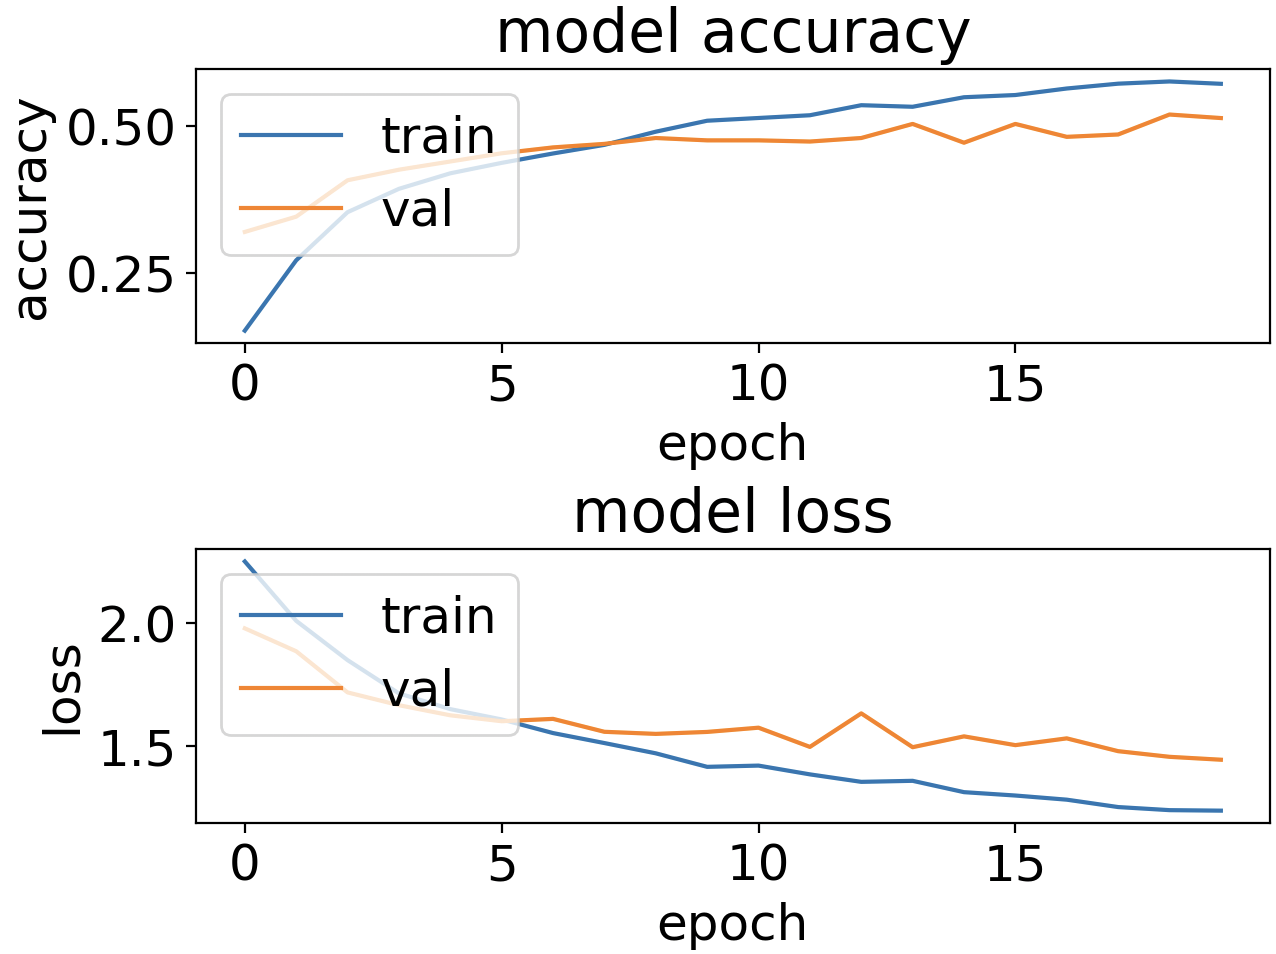
\includegraphics[width=.8\linewidth]{plot.png}
\end{center}
\captionof{figure}{A figure with two subplots, one showing the accuracy and one showing the loss of the model across epochs.}

The number of epochs a model should be trained with can be considered a hyper parameter which needs fine tuning to produce the best results. Too low an epoch will lead to underfitting and too high will lead to overfitting. By plotting the accuracy/loss of the model across a number of epochs, we can deduce the correct number of epochs to train for and what amounts of epochs lead to underfitting or overfitting. A big gap in training and validation lines can be a symptom of overfitting.

From the plot in figure 4 we can deduce that between 10-15 epochs our model begins to stagnate slightly, which could be a symptom of overfitting. It seems that an epoch of 10 might be the best amount.

\subsection{(ii)(b)(iii)}
In this part we trained several models, all with the same convnet but each being trained on a different amount of training points (5k, 10k, 20k, 40k). The time it took for each model to finish training was as follows:
\begin{center}
5k training points : 20 seconds

10k training points : 37 seconds

20k training points : 76 seconds

40k training points : 156 seconds
\end{center}

\begin{figure} [H]
\centering
\begin{subfigure}{.49\linewidth}
  \centering
  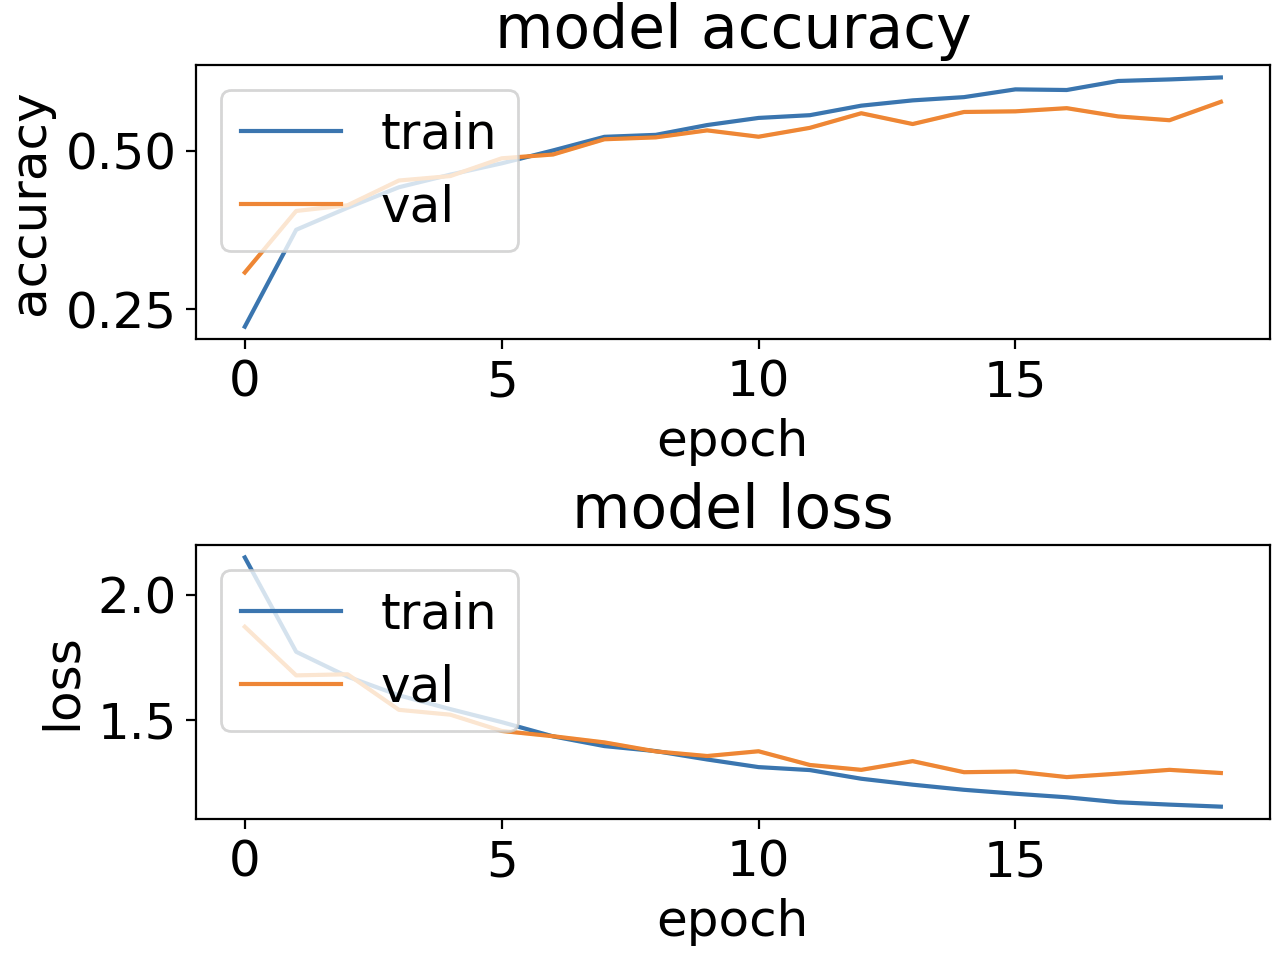
\includegraphics[width=\linewidth, height=6cm]{10k.png}
  \caption{Model accuracy/loss with 10k training points.}
  \label{fig:sub1}
\end{subfigure}%
\begin{subfigure}{.49\textwidth}
  \centering
  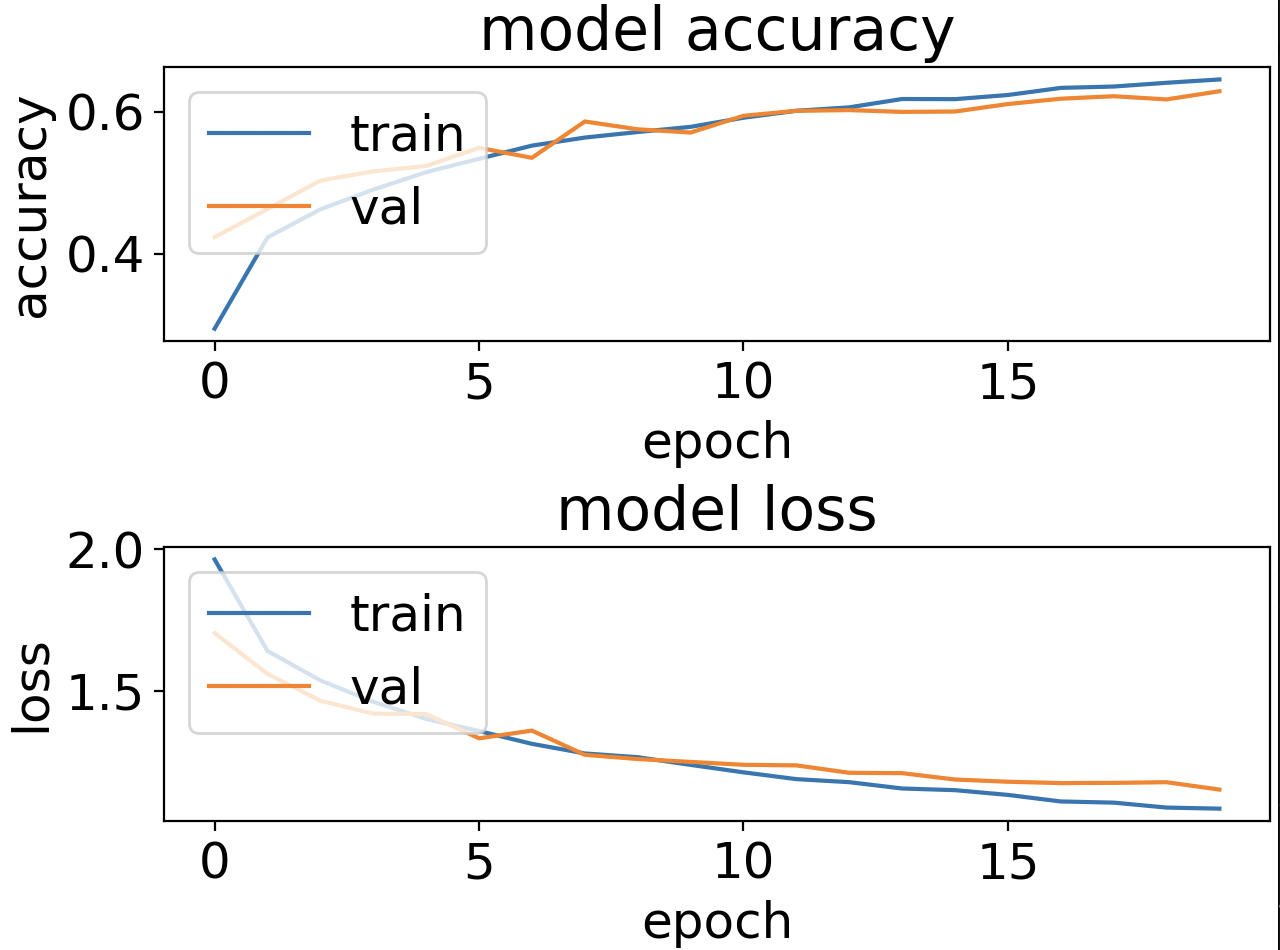
\includegraphics[width=\linewidth, height=6cm]{20k.png}
  \caption{Model accuracy/loss with 20k training points.}
  \label{fig:sub2}
\end{subfigure}
\label{fig:test}
\begin{subfigure}{.5\linewidth}
  \centering
  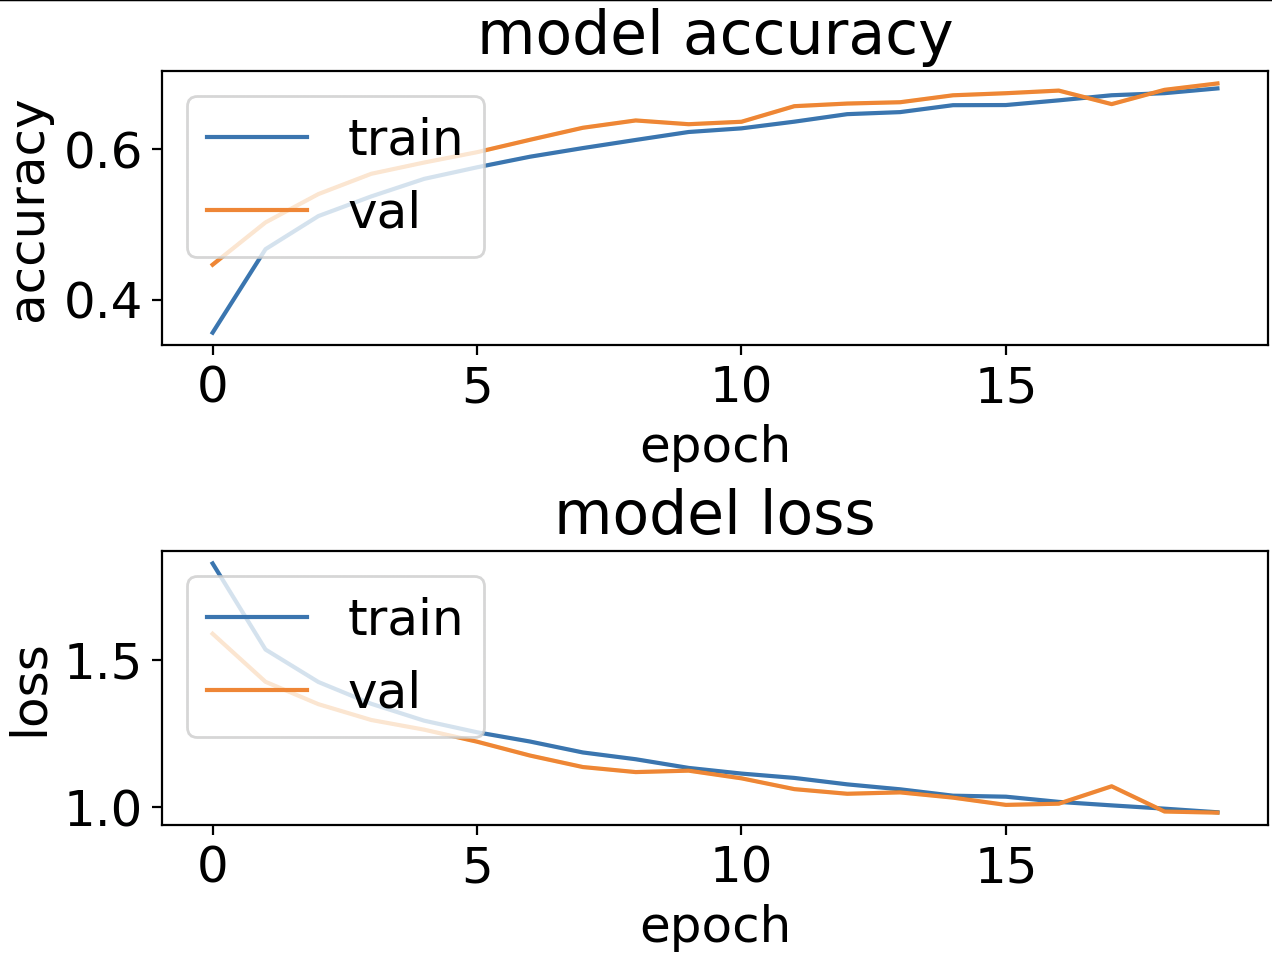
\includegraphics[width=\linewidth, height=6cm]{40k.png}
  \caption{Model accuracy/loss with 40k training points.}
  \label{fig:sub3}
\end{subfigure}%
\caption{A figure with three subfigures, each containing a visualization of model accuracy/loss across epochs. Each subfigure is trained on a different number of training points. }
\label{fig:test}
\end{figure}

The time it takes to train each model is doubled each time the amount of training data is doubled.

Each model is evaluated using f1 scores. The model trained on 5k points has an accuracy of 0.62 on training data and 0.50 on testing data. The model with 10k has an accuracy of 0.67 and 0.56 on training and testing respectively. The model with 20k has 0.70 and 0.63, and the model with 40k has 0.73 and 0.68. As the amount of training points rise, the accuracies of the models on both the training and testing rises too. The accuracy on training data is always higher than that of the testing data, though the gap between the two decreases with more training points.

Looking at figure 5, the more training points used the more the train and val lines converge and overlap. This means that the data is not overfitting like it was with only 5k training points. This makes sense as the more data a model sees, the more generalized it becomes.  

\subsection{(ii)(b)(iv)}

The softmax output layer is the final layer in a convnet, it translates the output of the network from real numbers into a probability distribution over the possible outcomes. L1 is a penalty added to the loss function of this layer that reduces the weights of parameters in a model to reduce overfitting. The higher the L1 penalty, the more the weights are reduced. 

\begin{figure} [H]
\centering
\begin{subfigure}{.49\linewidth}
  \centering
  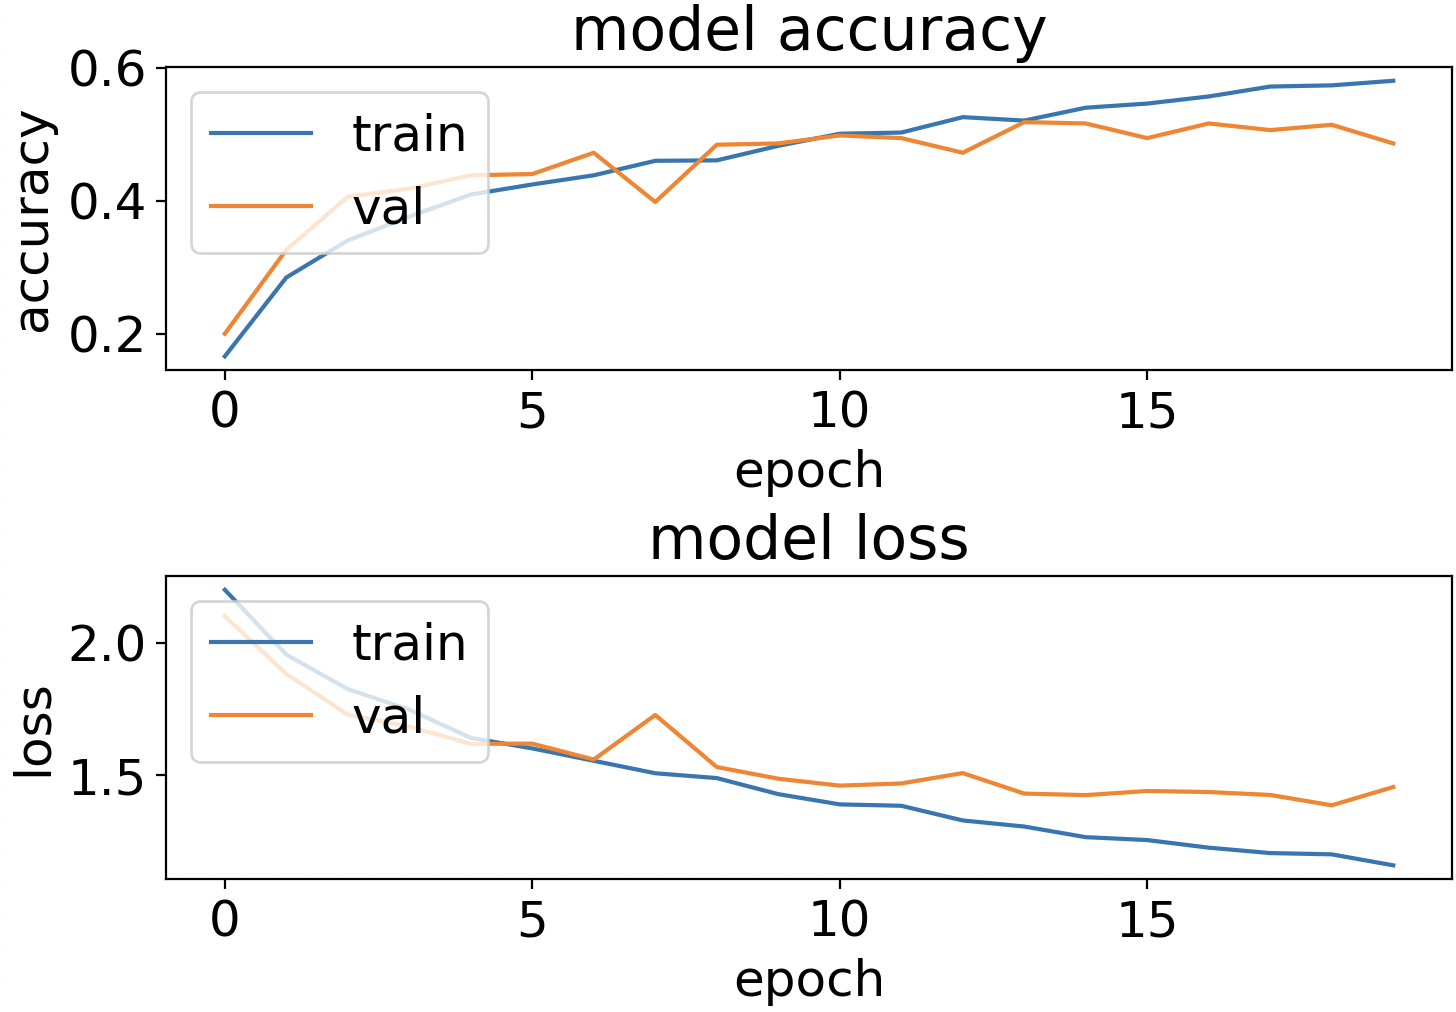
\includegraphics[width=\linewidth, height=6cm]{l0.png}
  \caption{Model accuracy/loss with L1 of 0.}
  \label{fig:sub1}
\end{subfigure}%
\begin{subfigure}{.49\textwidth}
  \centering
  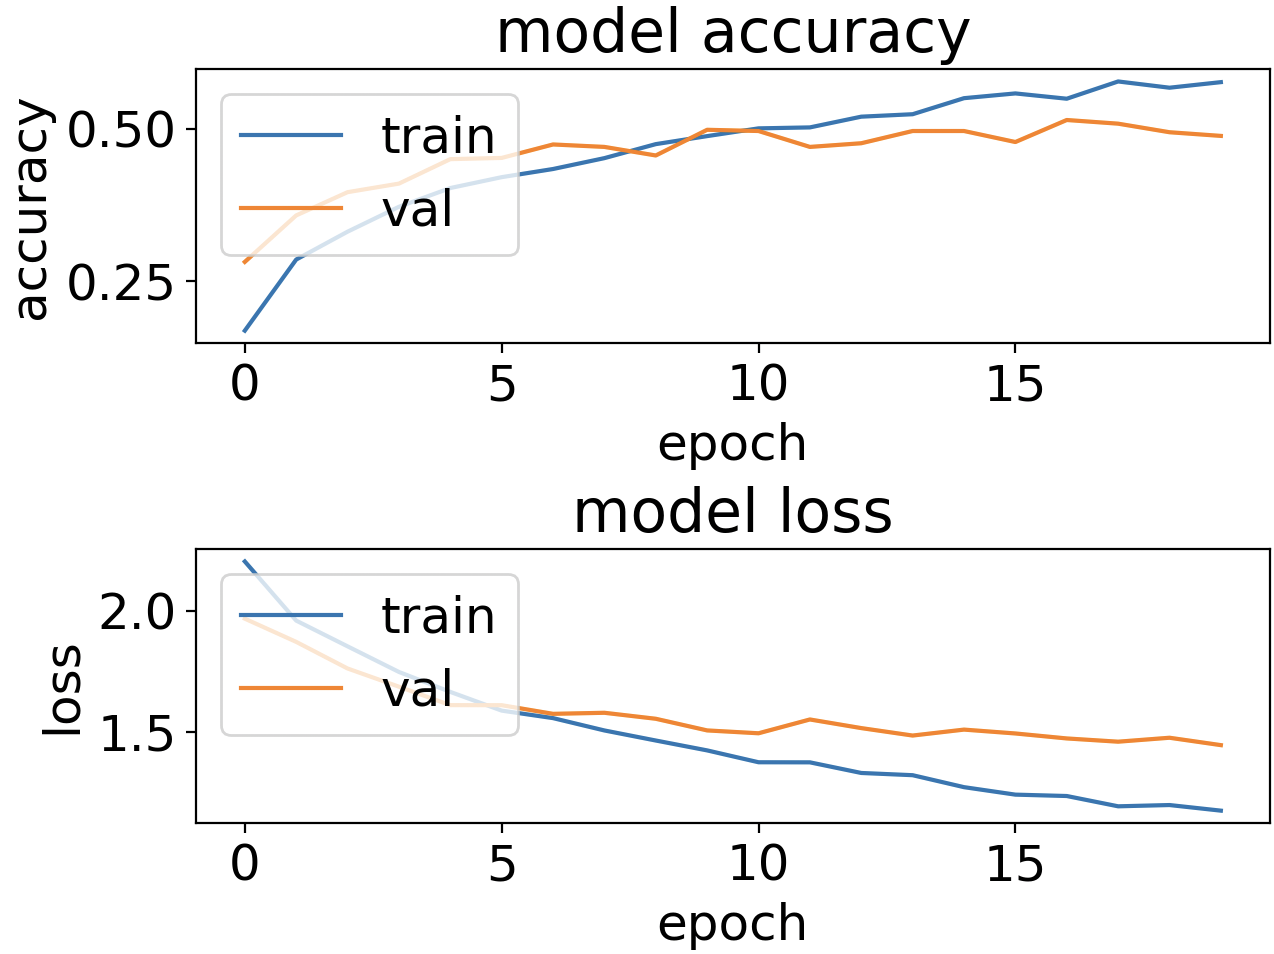
\includegraphics[width=\linewidth, height=6cm]{lsmall.png}
  \caption{Model accuracy/loss with L1 of 0.0000001.}
  \label{fig:sub2}
\end{subfigure}
\label{fig:test}
\begin{subfigure}{.5\linewidth}
  \centering
  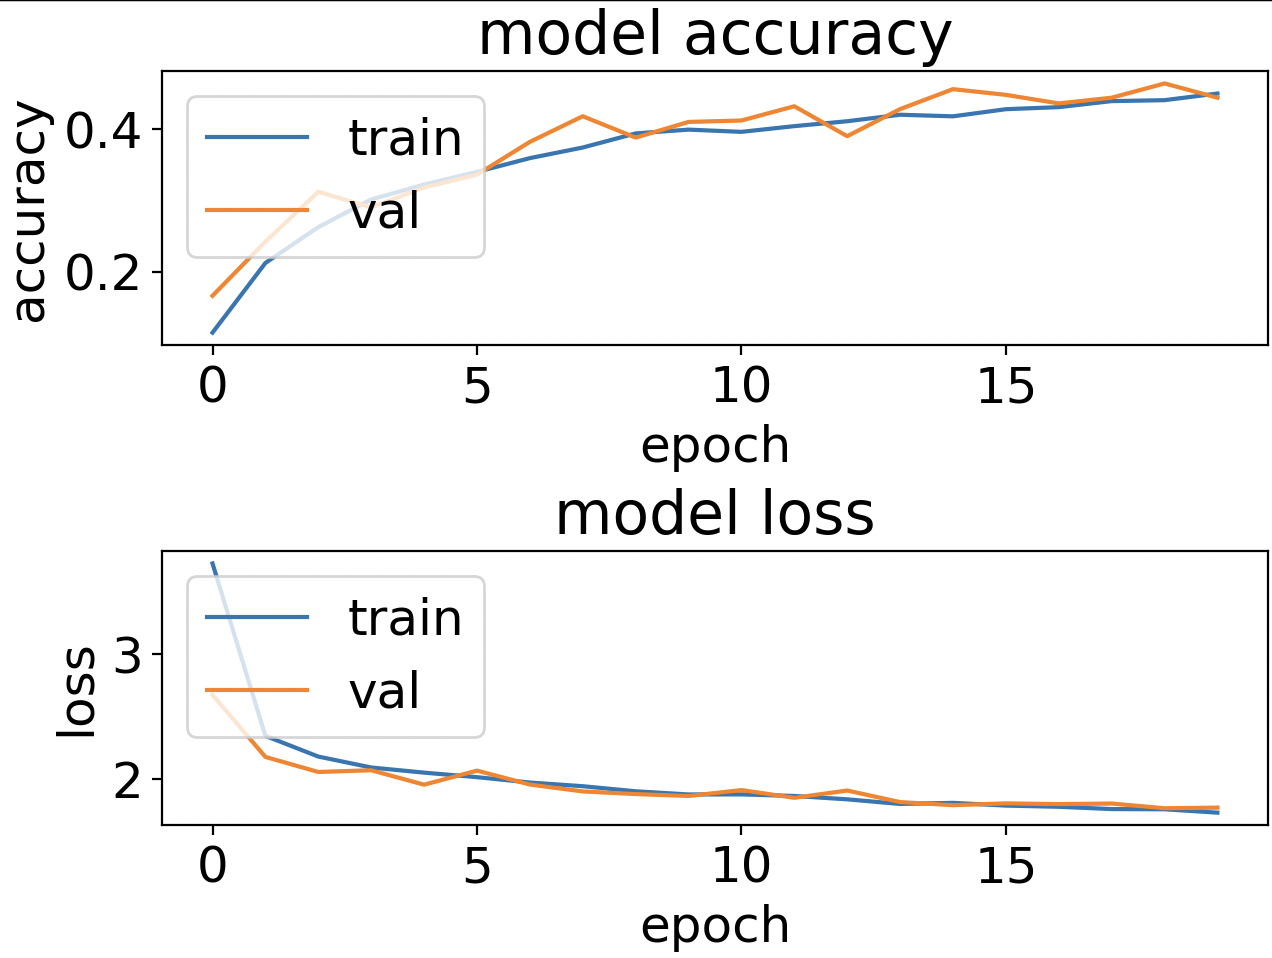
\includegraphics[width=\linewidth, height=6cm]{l5.png}
  \caption{Model accuracy/loss with L1 of 0.005.}
  \label{fig:sub3}
\end{subfigure}%
\begin{subfigure}{.5\linewidth}
  \centering
  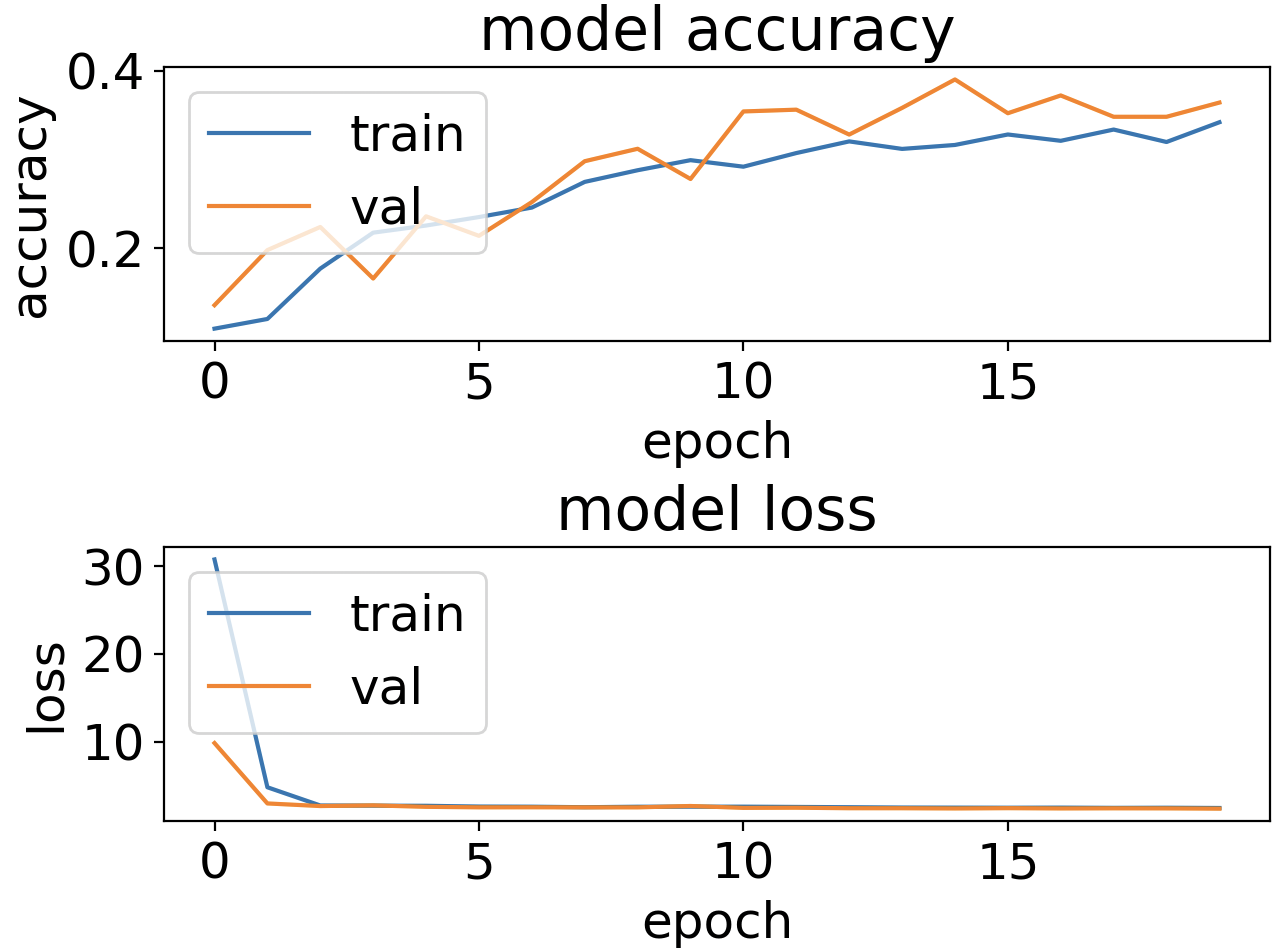
\includegraphics[width=\linewidth, height=6cm]{l1.png}
  \caption{Model accuracy/loss with L1 of 0.1.}
  \label{fig:sub3}
\end{subfigure}%
\caption{A figure with four subfigures, each containing a visualization of model accuracy/loss across epochs. Each subfigure has a different L1 Regularisation. }
\label{fig:test}
\end{figure}

The different penalties I chose were 0, 0.0000001, 0.005, and 0.1. I chose these penalties as they represent a wide spread both below and above the default penalty of 0.001. The f1 scores for each of the models in both training and testing were as follows:
\begin{center}
L1 of 0 : 0.62, 0.50

L1 of 0.0000001 : 0.64, 0.50

L1 of 0.005 : 0.49, 0.45

L1 of 0.1 : 0.35, 0.35
\end{center}
As the penalties became bigger, accuracy became much lower in both training and testing data. The difference between the accuracy on training and testing became much smaller however. These large penalties would have reduced a lot of parameters to 0, therefore leading to the model being underfit and losing accuracy.

Looking at the graphs in figure 6, we can see large penalties greatly increased the amount of loss the model goes through in the first few epochs. The models with smaller penalties seem to be slightly overfit as we can see on the graphs for accuracy they have a large difference between their train and val lines.

When comparing L1 regularization with increasing amount of training points as a tool to prevent overfitting, I would say the latter is more effective. L1 regularization is finicky, too small or too large of a penalty can harm your models results and it requires a lot of fine tuning to get correct. Whereas increasing the amount of training points always helps to prevent overfitting, there is no way for too many training points to harm your model. Though, even if more effective, it can sometimes be better to rely on L1 regularization over training points as an anti-overfitting measure. More data points means more time and power needed to train models, not to mention getting that amount of data in the first place. Changing the penalty, however, does not affect the time it takes to train. So even though adding more training points is more effective, it is often more efficient to change the L1 penalty.

\subsection{(ii)(c)(i)}
\begin{lstlisting}
	model.add(Conv2D(16, (3,3), padding='same', input_shape=x_train.shape[1:],activation='relu'))
	model.add(Conv2D(16, (3,3), padding='same', activation='relu'))
	model.add(MaxPooling2D(pool_size=(2, 2)))
	model.add(Conv2D(32, (3,3), padding='same', activation='relu'))
	model.add(Conv2D(32, (3,3), padding='same', activation='relu'))
	model.add(MaxPooling2D(pool_size=(2, 2)))
	model.add(Dropout(0.5))
	model.add(Flatten())
	model.add(Dense(num_classes, activation='softmax',kernel_regularizer=regularizers.l1(0.001)))
\end{lstlisting}

Above is the new structure for the Convnet, now instead of using Conv2d layers with increased stride to downsize there are now Max pooling layers. These pool layers have a pool size on (2,2) and a stride of (2x2), meaning there will be no overlap. Everything else about the architecture stays the same.

Max pooling layers take an input of size (H x W x D) and output of size (H1 x W1 x D), where H1 $< $ H and W1 $<$ W. This is achieved by taking a pooling block (in our case of size 2 by 2), and moving along the input with a stride usually the same size as the pooling block(so for our case 2 x 2). At each point, the largest number in the pool block and only the largest is transcribed into the output.

\subsection{(ii)(c)(ii)}
\begin{center}
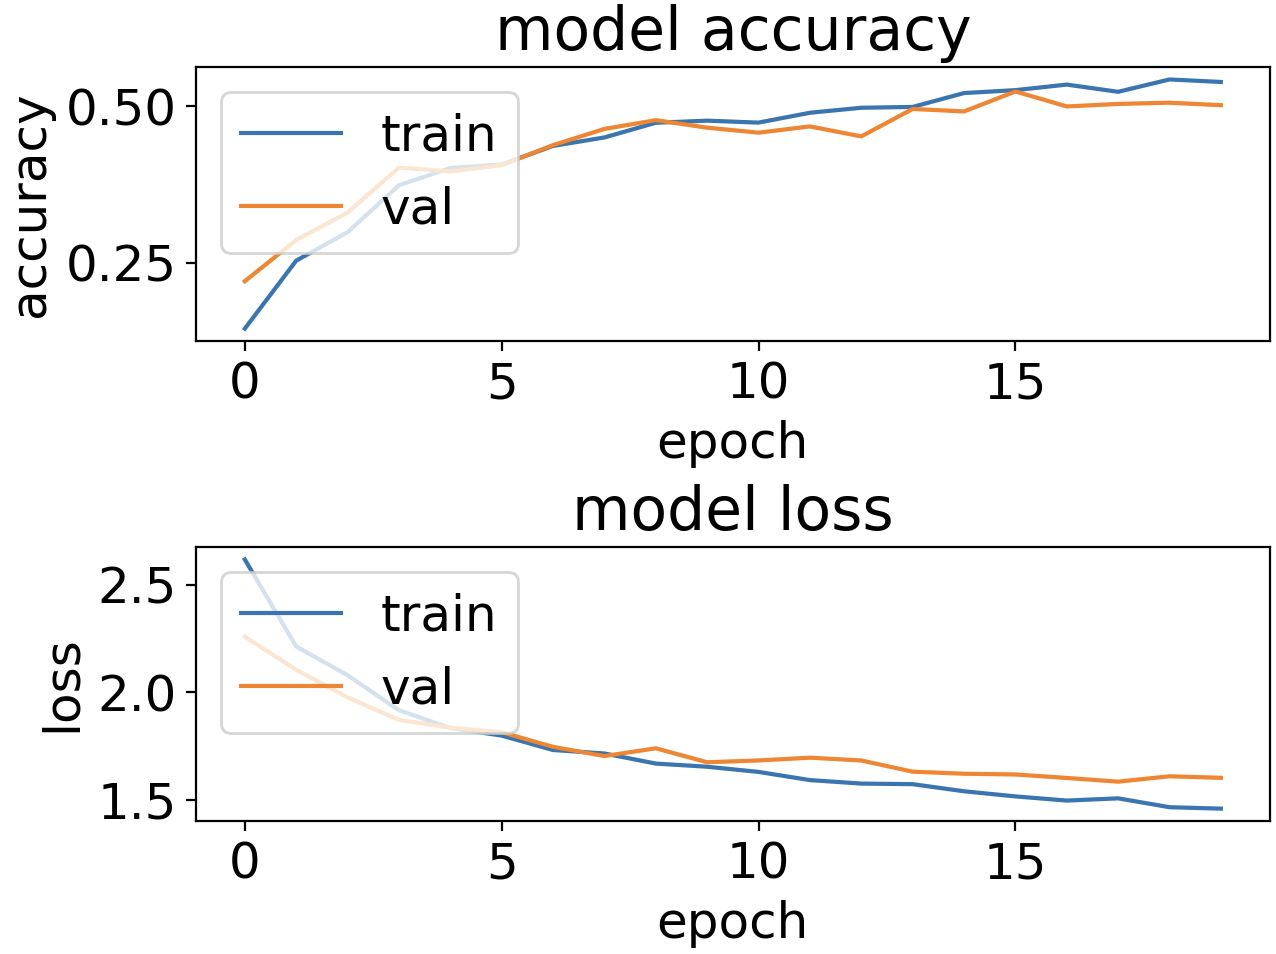
\includegraphics[width=.8\linewidth]{pool.png}
\end{center}
\captionof{figure}{A figure with two subplots, one showing the accuracy and one showing the loss of the model across epochs. This is for a model using Max pooling to reduce size. }

This architecture has 37,146 parameters, this is the same as the previous model. The max pool layers themselves have 0 parameters as there is no complex function to get the maximum. The additional Conv2D layers added made up the difference.

With this new architecture, the model took 36 seconds to train on 5k training points. This is longer than the downstride model took. This is because we have added another convolution layer with a stride of 1 in addition to the pooling layer, so despite max pooling being generally faster than down-striding this additional layer eats up the difference and more.

The max-pool model's f1 score for training data was 0.61, and for testing data is was 0.53. Compared to the downstride models which was 0.64 and 0.50 respectively. The max-pool model performed worst in training accuracy but slightly better in testing accuracy. The lower training accuracy could be because max-pools inherently cause the model to use less information than when using strides to downsize.

\section{Appendix}
\lstinputlisting[language=Python]{../main.py}
\end{document}



